%
% Selección de comparación de desempeño.
% Implementación de programa tokenizador, reporte técnico.
%
% Proyecto Lovelace.
%

\subsection{Comparación de desempeño}
\label{sec:comparacion}

Como se indicó en la introducción de este trabajo, la tokenización digital es un
proceso relativamente nuevo y la mayoría de los proveedores de este servicio
aprovechan la confusión y desinformación existente para atraer a clientes
potenciales, pues pocos comparten la manera en que crean sus \glspl{gl:token}.
Esta sección busca resarcir un poco el daño, presentado una comparación entre
los tiempos de respuesta de tokenización y detokenización de los algoritmos
implementados.

En la tabla \ref{tabla:tiempos_tokenizacion} se puede observar el tiempo
promedio que le toma a cada algoritmo hacer el número de tokenizaciones o
detokenizaciones señaladas en el encabezado. Los algoritmos están
divididos en reversibles y no reversibles, pues, dadas sus características, no
sería muy parejo compararlos entre sí; por ejemplo, basta hacer una consulta
en la base de datos para hacer la detokenización en los algoritmos
irreversibles; mientras que en los reversibles hay que hacer el proceso inverso,
o uno equivalente, para poder obtener de nuevo el \gls{gl:pan}.

\begin{table}
  \begin{center}
  \begin{tabular}{cc|c|c|c|c|c|c|}
    \cline{3-8}
    & & \multicolumn{2}{c|}{100 oper.} & \multicolumn{2}{c|}{1K oper.}
      & \multicolumn{2}{c|}{10K oper.} \\
      \cline{3-8}

    & & Tok. & Detok. & Tok. & Detok. & Tok. & Detok. \\
    \hline
    \multicolumn{1}{|c }{ \multirow{2}{*}{Reversibles} } &
    \multicolumn{1}{|c|}{BPS} & 7.247 $m$s  & 6.990 $m$s  & 68.514 $m$s
      & 68.566 $m$s & 714.336 $m$s & 674.571 $m$s \\ \cline{2-8}
    \multicolumn{1}{ |c  }{}                        &
    \multicolumn{1}{|c|}{FFX} & 5.627 $m$s  & 5.516 $m$s  & 49.738 $m$s
      & 49.550 $m$s & 487.529 $m$s & 340.749 $m$s \\
    \hline

    \multicolumn{1}{|c }{ \multirow{3}{*}{Irreversibles} } &
    \multicolumn{1}{|c|}{TKR}   & 6.573 s  & 37.623 $m$s  & 70.116 s
      & 441.815$m$s & 882.695 s & 4.976 s \\ \cline{2-8}
    \multicolumn{1}{ |c  }{}                        &
    \multicolumn{1}{|c|}{AHR}   & 6.053 s  & 58.814 $m$s  & 65.631 s
      & 420.729$m$s & 735.405 s & 5.269 s \\ \cline{2-8}
    \multicolumn{1}{ |c  }{}                        &
    \multicolumn{1}{|c|}{DRBG}  & 6.718 s  & 40.265 $m$s  & 71.082 s
      & 436.753$m$s & 826.403 s & 7.226 s \\ \hline
  \end{tabular}

  \caption{Comparación de tiempos de tokenización de los
    algoritmos implementados.}
  \label{tabla:tiempos_tokenizacion}
\end{center}
\end{table}

Los datos de la tabla \ref{tabla:tiempos_tokenizacion} fueron utilizados para
crear una serie de gráficas: en la figura \ref{figura:tok_todos} se comparan los
tiempos de tokenización y detokenización de todos los algoritmos, tanto
reversibles como irreversibles; la velocidad de los algoritmos reversibles es
notoria, en especial al momento de la operación de tokenización. Posteriormente,
en la figura \ref{figura:tok_rev}, se compararon solo los algoritmos reversibles
(\hyperref[sec:bps]{BPS} y \hyperref[sec:ffx]{FFX}), siendo el segundo el más
rápido de los dos; especialmente cuando se realizan operaciones de
detokenización. Finalmente, se compararon los tiempos para los algoritmos
irreversibles en las gráficas de la figura \ref{figura:tok_irrev}: durante las
operaciones de tokenización, aunque están relativamente cerrados los tiempos,
\hyperref[sec:ahr]{AHR} queda como el más rápido de los tres, mientras que
\hyperref[sec:drbg_lista]{DRBG} queda en segundo lugar; es menester recordar
porqué estos algoritmos toman más tiempo: \hyperref[sec:ahr]{AHR} utiliza
\gls{gl:cifrado_caminata_ciclica}, y, al generar un \gls{gl:token}, consulta la
base de datos, pues permite tener más de un \gls{gl:token} por \gls{gl:pan};
además, tanto \hyperref[sec:tkr]{TKR2} como \hyperref[sec:drbg_lista]{DRBG}
necesitan bits pseudoaleatorios, y si el generador de bits pseudoaleatorios
tarda en obtenerlos, los algoritmos se ven afectados; finalmente, en las
operaciones de detokenización, \hyperref[sec:tkr]{TKR2} es el más rápido de
todos, mientras que \hyperref[sec:drbg_lista]{DRBG} queda como el más lento.

\begin{figure}
  \centering
  \begin{subfigure}{1\textwidth}
    \begin{center}
      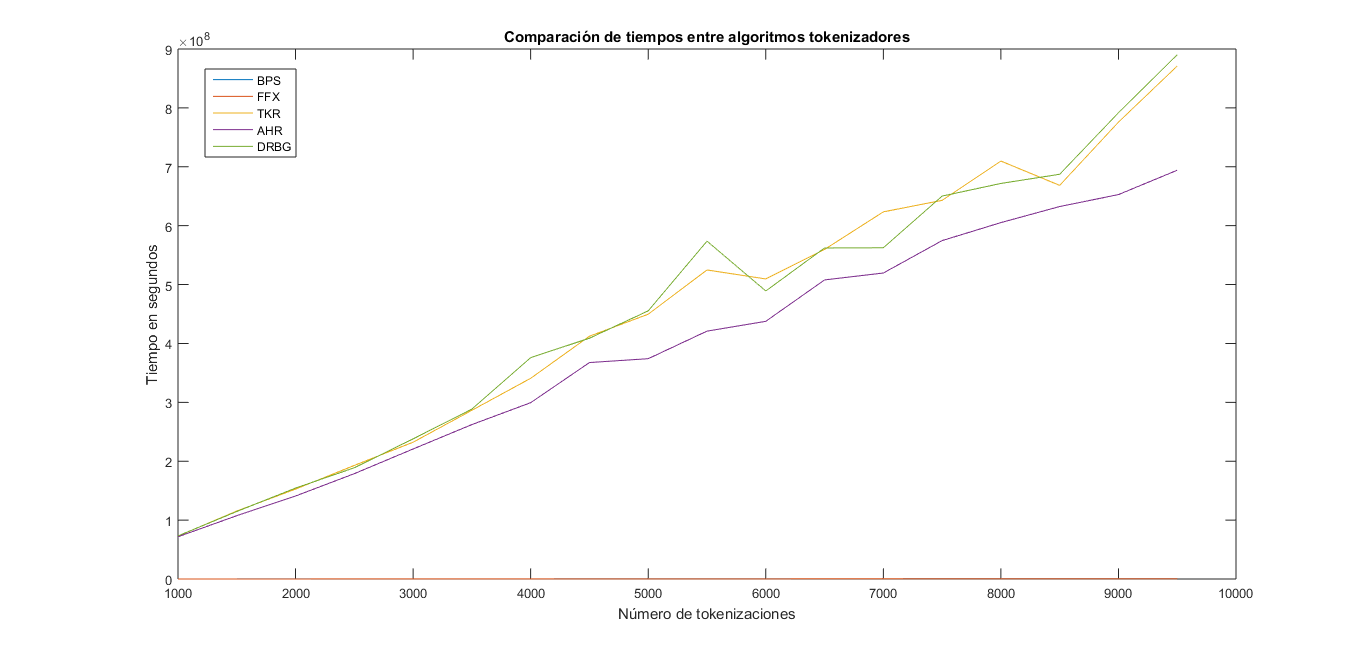
\includegraphics[width=1\linewidth]{diagramas/tok_todos}
      \caption{Tiempos de tokenización.}
    \end{center}
  \end{subfigure}
  \begin{subfigure}{0.9\textwidth}
    \begin{center}
      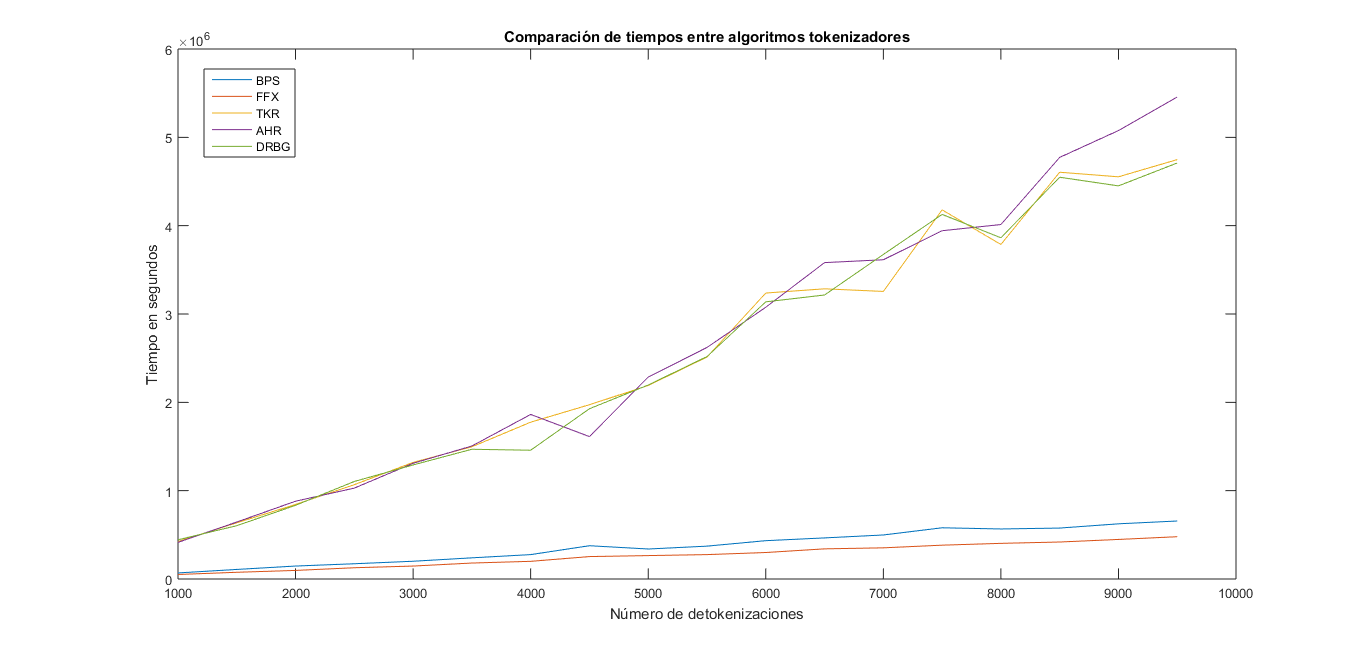
\includegraphics[width=1\linewidth]{diagramas/detok_todos}
      \caption{Tiempos de detokenización.}
    \end{center}
  \end{subfigure}
  \caption{Comparación de tiempos entre algoritmos tokenizadores.}
  \label{figura:tok_todos}
\end{figure}

\begin{figure}
  \centering
  \begin{subfigure}{1\textwidth}
    \begin{center}
      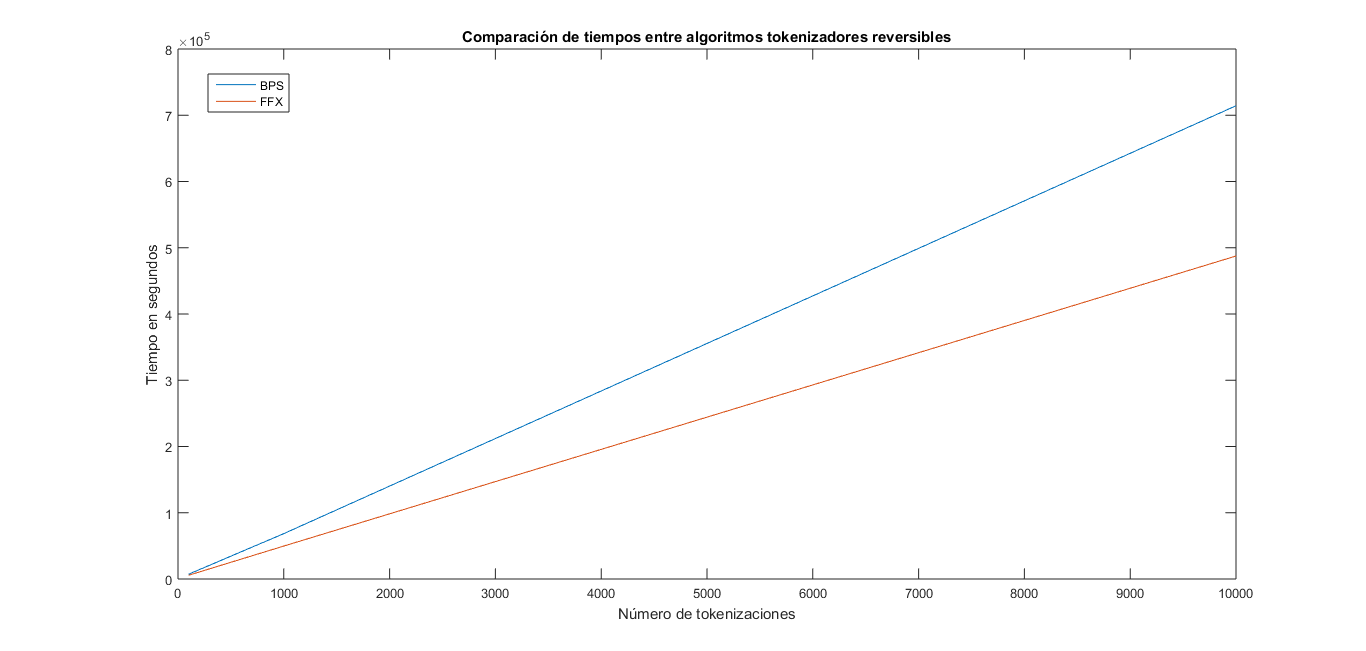
\includegraphics[width=1\linewidth]{diagramas/tok_rev}
      \caption{Tiempos de tokenización.}
    \end{center}
  \end{subfigure}
  \begin{subfigure}{0.9\textwidth}
    \begin{center}
      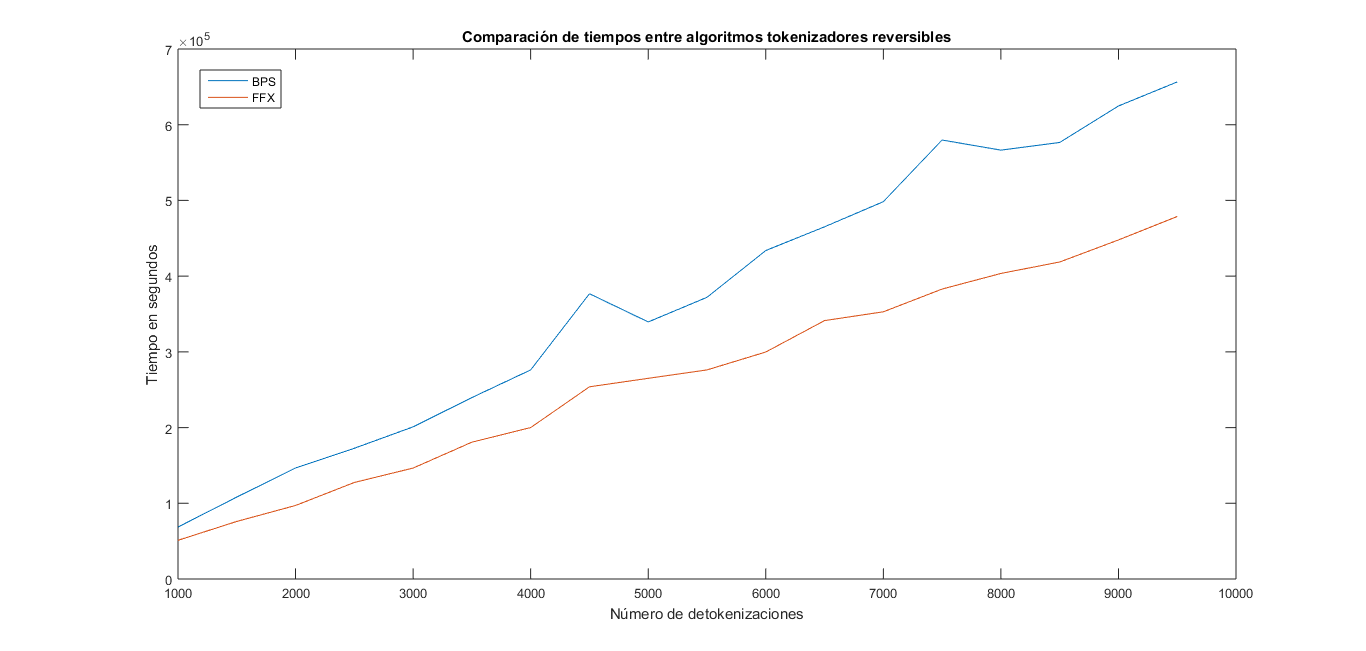
\includegraphics[width=1\linewidth]{diagramas/detok_rev}
      \caption{Tiempos de detokenización.}
    \end{center}
  \end{subfigure}
  \caption{Comparación de tiempos entre algoritmos tokenizadores reversibles.}
  \label{figura:tok_rev}
\end{figure}

\begin{figure}
  \centering
  \begin{subfigure}{1\textwidth}
    \begin{center}
      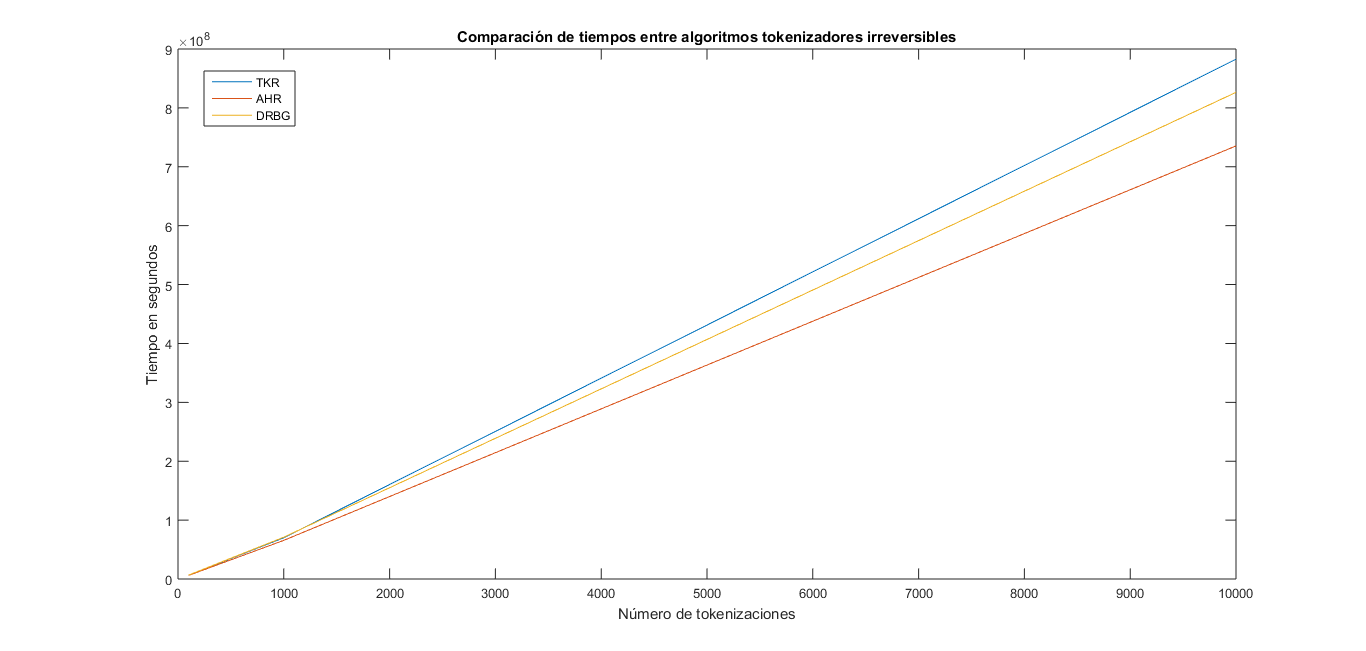
\includegraphics[width=1\linewidth]{diagramas/tok_irrev}
      \caption{Tiempos de tokenización.}
    \end{center}
  \end{subfigure}
  \begin{subfigure}{0.9\textwidth}
    \begin{center}
      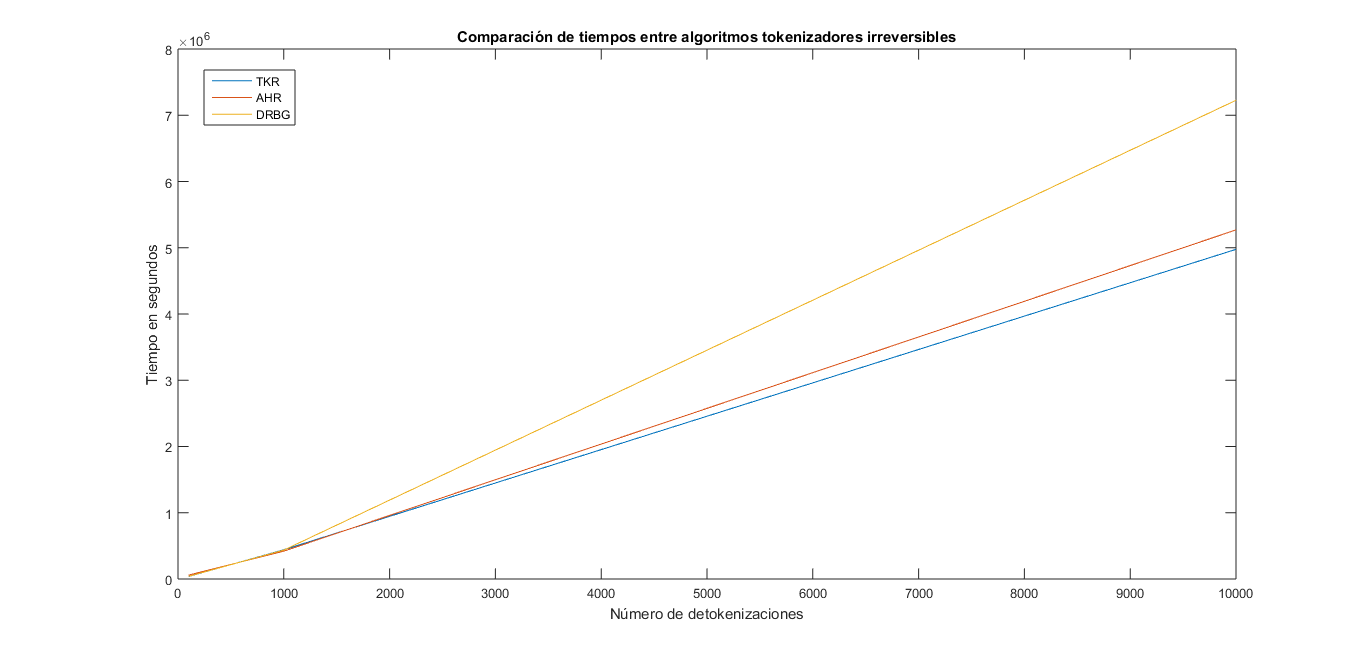
\includegraphics[width=1\linewidth]{diagramas/detok_irrev}
      \caption{Tiempos de detokenización.}
    \end{center}
  \end{subfigure}
  \caption{Comparación de tiempos entre algoritmos tokenizadores irreversibles.}
  \label{figura:tok_irrev}
\end{figure}
